\documentclass[a4paper,11pt]{article}
\usepackage{amsmath,amsthm,amsfonts,amssymb,amscd,amstext,vmargin,graphics,graphicx,tabularx,multicol} 
\usepackage[francais]{babel}
\usepackage[utf8]{inputenc}  
\usepackage[T1]{fontenc} 
\usepackage{pstricks-add,tikz,tkz-tab,variations}
\usepackage[autolanguage,np]{numprint} 

\setmarginsrb{1.5cm}{0.5cm}{1cm}{0.5cm}{0cm}{0cm}{0cm}{0cm} %Gauche, haut, droite, haut
\newcounter{numexo}
\newcommand{\exo}[1]{\stepcounter{numexo}\noindent{\bf Exercice~\thenumexo} : \marginpar{\hfill /#1}}
\reversemarginpar


\newcounter{enumtabi}
\newcounter{enumtaba}
\newcommand{\q}{\stepcounter{enumtabi} \theenumtabi.  }
\newcommand{\qa}{\stepcounter{enumtaba} (\alph{enumtaba}) }
\newcommand{\initq}{\setcounter{enumtabi}{0}}
\newcommand{\initqa}{\setcounter{enumtaba}{0}}

\newcommand{\be}{\begin{enumerate}}
\newcommand{\ee}{\end{enumerate}}
\newcommand{\bi}{\begin{itemize}}
\newcommand{\ei}{\end{itemize}}
\newcommand{\bp}{\begin{pspicture*}}
\newcommand{\ep}{\end{pspicture*}}
\newcommand{\bt}{\begin{tabular}}
\newcommand{\et}{\end{tabular}}
\renewcommand{\tabularxcolumn}[1]{>{\centering}m{#1}} %(colonne m{} centrée, au lieu de p par défault) 
\newcommand{\tnl}{\tabularnewline}

\newcommand{\bmul}[1]{\begin{multicols}{#1}}
\newcommand{\emul}{\end{multicols}}

\newcommand{\trait}{\noindent \rule{\linewidth}{0.2mm}}
\newcommand{\hs}[1]{\hspace{#1}}
\newcommand{\vs}[1]{\vspace{#1}}

\newcommand{\N}{\mathbb{N}}
\newcommand{\Z}{\mathbb{Z}}
\newcommand{\R}{\mathbb{R}}
\newcommand{\C}{\mathbb{C}}
\newcommand{\Dcal}{\mathcal{D}}
\newcommand{\Ccal}{\mathcal{C}}
\newcommand{\mc}{\mathcal}

\newcommand{\vect}[1]{\overrightarrow{#1}}
\newcommand{\ds}{\displaystyle}
\newcommand{\eq}{\quad \Leftrightarrow \quad}
\newcommand{\vecti}{\vec{\imath}}
\newcommand{\vectj}{\vec{\jmath}}
\newcommand{\Oij}{(O;\vec{\imath}, \vec{\jmath})}
\newcommand{\OIJ}{(O;I,J)}


\newcommand{\reponse}[1][1]{%
\multido{}{#1}{\makebox[\linewidth]{\rule[0pt]{0pt}{20pt}\dotfill}
}}

\newcommand{\titre}[5] 
% #1: titre #2: haut gauche #3: bas gauche #4: haut droite #5: bas droite
{
\noindent #2 \hfill #4 \\
#3 \hfill #5

\vspace{-1.6cm}

\begin{center}\rule{6cm}{0.5mm}\end{center}
\vspace{0.2cm}
\begin{center}{\large{\textbf{#1}}}\end{center}
\begin{center}\rule{6cm}{0.5mm}\end{center}
}



\begin{document}
\pagestyle{empty}
\titre{Interrogation: Additions, soustractions }{Nom :}{Prénom :}{Classe}{Date}



\vspace*{0.5cm}
\begin{flushleft}
\begin{tabular}{|m{9.5cm}|m{1.25cm}|m{1.25cm}|m{1.25cm}|m{1.25cm}|m{1.25cm}|}
\hline 
\textbf{Compétences} & \begin{center}
\textbf{N.E.}
\end{center} & \begin{center}
\textbf{M.I.}
\end{center} & \begin{center}
\textbf{M.F.}
\end{center}  & \begin{center}
\textbf{M.S.}
\end{center} & \begin{center}
\textbf{T.B.M.}
\end{center} \\ 
\hline 
Je dois savoir maitriser le vocabulaire de l'addition et de la soustraction &  &  & & &\\
\hline 
Je dois savoir additionner des nombres entiers et des nombres décimaux (calcul mental, posé, instrumenté) &  &  & & &\\
\hline
 Je dois savoir calculer une expression en ligne de manière astucieuse&  &  & & &\\ 
\hline
Je dois savoir soustraire des nombres entiers et des nombres décimaux (calcul mental, posé ou instrumenté)&  &  & & &\\ 
\hline
\end{tabular} 
\end{flushleft}

\textit{N.E = Non évalué ; M.I. = Maîtrise insuffisante ; M.F. = Maîtrise fragile ; M.S. = Maîtrise satisfaisante ; T.B.M. = Très bonne maîtrise}\\



\exo{1} Question de cours : Écrire la définition qui concerne l'addition.\\
\reponse[4]\\


\exo{2.25} Poser et effectuer les opérations suivantes.\\

1 562,45 + 542,7 \hspace*{3cm} 1 583 + 284,5 + 603,99 \hspace*{3cm} 726,5 – 408,84\\

\vspace*{7cm}

\exo{2.25} Compléter les opérations suivantes.

\begin{center}
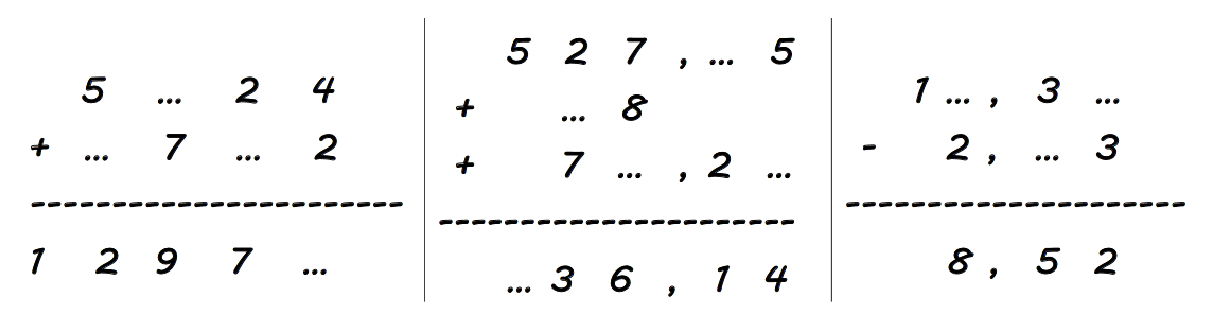
\includegraphics[scale=0.8]{exo1.eps} 
\end{center}

\newpage

\vspace*{0.3cm}

\exo{2} Calculer astucieusement les expressions suivantes à l'aide de la méthode vue en classe. Il faudra détailler les étapes de vos calculs.



\bmul{2}
 
 $L = 7,5 + 12,6 + 2,5 + 14,4 $\\
 \reponse[8]\\





\columnbreak


$B = 0,95 +125 + 18 + 6,8 + 1,05+75 + 3,2 $\\
 \reponse[8]\\


\emul


\vspace*{0.3cm}

\exo{2.5} Dans une papeterie, Mathilde achète un agenda à 7,96 euros, des bâtons de colle à 3,44 euros, des cahiers à 5,08 euros et un lot de stylo à 9,59 euros. \\

\initq \q  Déterminer un ordre de grandeur de la somme totale qu'elle va payer.\\
\reponse[3]\\

\q  Calculer le montant total de ses achats. Vous pourrez poser au brouillon les opérations. Vous donnerez votre réponse avec un calcul en ligne.\\
\reponse[5]\\

\q Mathilde paye avec deux billets de 20 euros. Combien va-t-on lui rendre?\\
\reponse[4]\\

\exo \\
BONUS\\

Une bouteille de vin coute 20 euros (bouteille + vin). Le vin coute 19 euros de plus que la bouteille.\\
Combien coûte la bouteille vide ? \\
\reponse[4]\\


\end{document}
